\section{实验}
在上一节,我们证明了基于均匀采样的算法在谱聚类上有更紧的理论界,另一方面,算法\ref{alg: uniform_wkk}能把谱聚类$O(n^3)$的时间复杂度降到$O(s^2+ns)$。在本节,我们就实现这一算法,用实验来体现该算法在实践中可以又快又好的解决谱聚类问题。这里,我们在6个数据集\footnote{下载地址 \url{http://www.escience.cn/people/chenxiaojun/index.html}}上做实验,数据集描述见表\ref{tab:datasets_spectral_clustering}。
\begin{table}[h]
	\caption{数据量$n$, 类数目$k$, 维度$d$}
	\label{tab:datasets_spectral_clustering}
	\begin{tabular}{ccccc}
		\toprule
		数据集 & 名字 & $n$ & $d$ & $k$ \\
		\midrule
		$D_1$ & segment &2310 & 19 & 7 \\
		$D_2$ & MnistData-05 &3495 &784 & 10 \\
		$D_3$ & MnistData-10 &6996 & 784 & 10 \\
		$D_4$ & isolet5 &7797 & 617 & 26 \\
		$D_5$ & USPS &9298 & 256 & 10 \\
		$D_6$ & letter-recognition &20000 & 16 & 26 \\
		\bottomrule
	\end{tabular}
\end{table}

参与实验的算法是算法\ref{alg: uniform_wkk},其中$\alpha$近似算法是带权kernel $k$-means++,实验基准算法是带权kernel $k$-means++后接带权kernel Lloyd(即算法\ref{alg: uniform_wkk}不采样的版本)。实验中相似度矩阵$A$的构建方式采用了文献\cite{chen2017scalable}的方法,anchor数目是数据点数目的20\%,算法\ref{alg: uniform_wkk}的采样数目也是数据点数目的20\%,两个算法的最大迭代次数都是30。由于随机性,算法\ref{alg: uniform_wkk}和基准算法在每个数据集上都会重复20次,取平均值汇报。Ncut和时间(秒)分别用来评价谱聚类聚类质量和聚类速度。

\begin{figure}[h]
    \subfloat[]{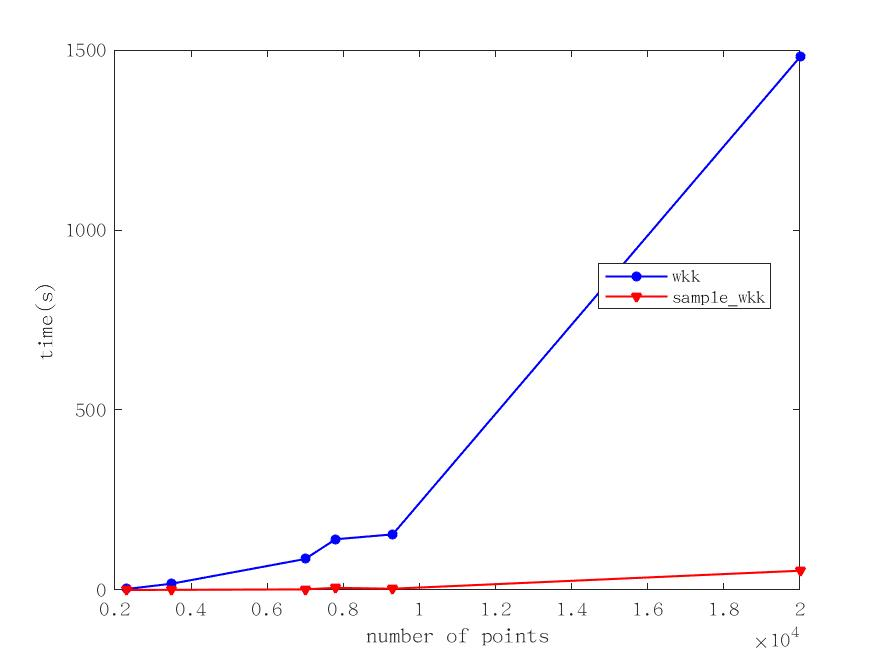
\includegraphics[width=0.5\linewidth]{sp-running_time.jpg}}
    \subfloat[]{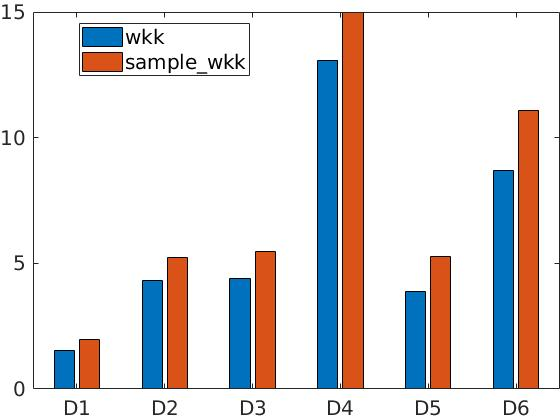
\includegraphics[width=0.5\linewidth]{sp-Ncuts.jpg}}
    \caption{谱聚类结果。(a)聚类所花时间(秒);(b)谱聚类的Ncut;}
    \label{fig: sp-experiments}
\end{figure}
结果见图\ref{fig: sp-experiments},从图中我们可以看出,基于采样的方法解决谱聚类的速度比不采样快了20~50倍,非常显著的加速了谱聚类的求解,另一方面,基于采样的方法的聚类质量又没有比不采样差太多,Ncut比不采样大了0.5~2.4,平均下来不超过不采样的25\%,较不采样而言,采样对聚类质量的影响不太显著,这验证了算法\ref{alg: uniform_wkk}在实践中可以又快又好的解决谱聚类问题。图\ref{fig: sp-experiments}中的数据列在表\ref{tab: res_spectral_cls}中。
\begin{table}[h]
	\caption{谱聚类Ncut和时间(时间在括号中,单位:秒)}
	\label{tab: res_spectral_cls}
	\begin{tabular}{ccc}
		\toprule
		数据集 & 带权kernel $k$-means & 采样的带权kernel $k$-means \\
		\midrule
		$D_1$ & 1.52(2.8) & 1.97(0.1) \\
		$D_2$ & 4.31(17.6) & 5.24(0.4) \\
		$D_3$ & 4.40(86.2) & 5.47(1.7) \\
		$D_4$ & 13.09(140.9) & 14.97(6) \\
		$D_5$ & 3.86(154.5) & 5.25(3.5) \\
		$D_6$ & 8.69(1480.6) & 11.10(53.6) \\
		\bottomrule
	\end{tabular}
\end{table}

